
\documentclass[a4paper,12pt]{article}
\usepackage{epstopdf}
\usepackage[utf8]{inputenc}
\usepackage[english]{babel}
\usepackage{enumerate}
\usepackage{mathtools}
\usepackage{hyperref}
\usepackage{float}
\usepackage[pdftex]{graphicx}   
\usepackage{multirow}
\usepackage{listings}
\lstset{
    language=matlab,
    basicstyle=\ttfamily
}

\title{TBMI26  \\
       Assignment 2}
\author{Martin Estgren \texttt{<mares480>}}
      
\begin{document}
 \pagenumbering{arabic}
    \maketitle % Generate.

\section{Boosting using the AdaBoost algorithm}

For the test we examine the performance of cascaded weak classifiers based on haar-features from a single classifier up to \textit{200}. We use \textit{400} samples for the training set, that is \textit{200} images of faces and \textit{200} of non-faces, and the rest of the data set for testing/validation.

\begin{figure}[H]
\centering
  \begin{minipage}[]{0.8\textwidth}
  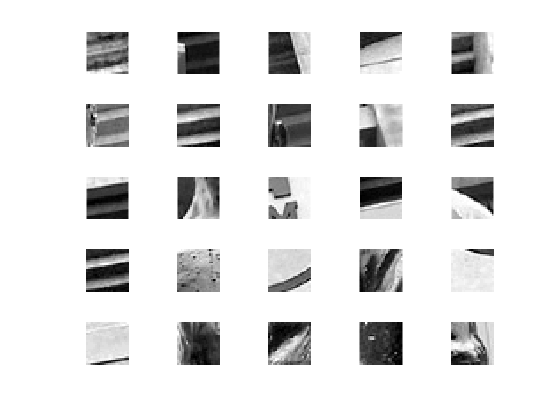
\includegraphics[width=\textwidth]{figures/sample_of_non_faces.png}
  \caption{Sample of faces}\label{fig:sample_data_set}

  \end{minipage}
    \begin{minipage}[]{0.8\textwidth}
  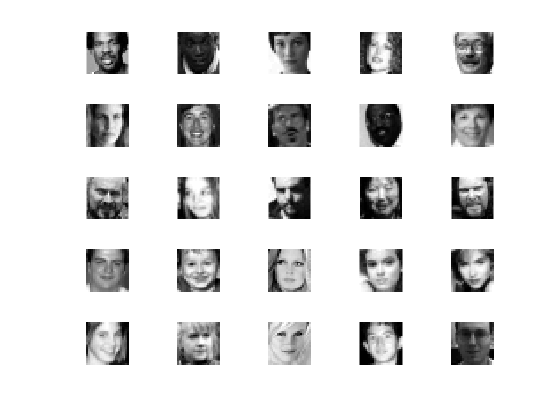
\includegraphics[width=\textwidth]{figures/sample_of_faces.png}
  \caption{Sample of non-faces}\label{fig:sample_data_set}

  \end{minipage}
\end{figure}
\begin{figure}[H]
\centering
\caption{Sample of haar-features}\label{fig:sample_haar_features}
  \begin{minipage}[]{0.8\textwidth}
  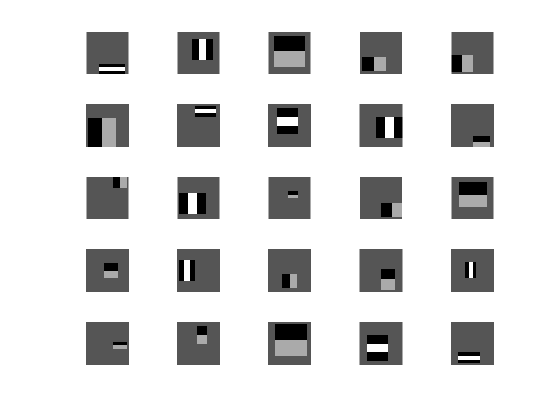
\includegraphics[width=\textwidth]{figures/sample_of_haar_features.png}
  \end{minipage}
\end{figure}

Below we can observe the error in accuracy given the number of weak classifiers for the training dataset. When we increase the number of classifiers the correct classification rate increases. Looking only at the training data we pick \textit{196} as the best number of classifiers.

\begin{figure}[H]
\centering
\caption{Training error given the number of weak classifiers}\label{fig:train_error}
  \begin{minipage}[]{0.80\textwidth}
  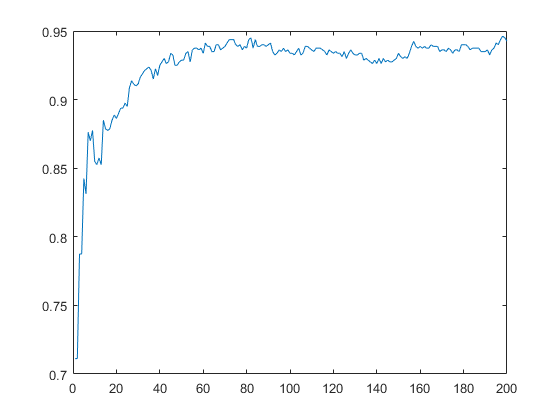
\includegraphics[width=\textwidth]{figures/train_error.png}
  \end{minipage}
\end{figure}

Below we can observe the error in accuracy given the number of weak classifiers for the testing/validation dataset. We can observe how we get diminishing returns in terms of accuracy when we have about 40 weak classifiers. We get the best accuracy when we have \textit{84} classifiers with an accuracy of \textit{0.8887}.

\begin{figure}[H]
\centering
\caption{Test error given the number of weak classifiers}\label{fig:test_error}
  \begin{minipage}[]{0.80\textwidth}
  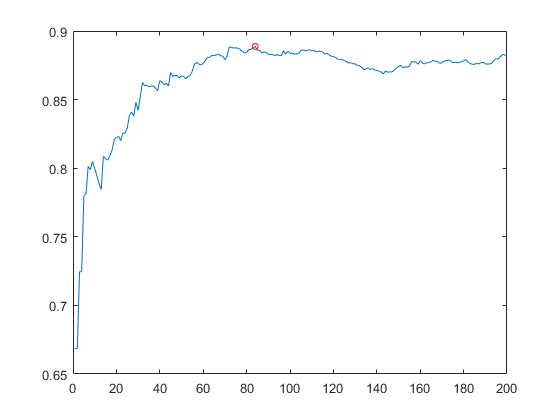
\includegraphics[width=\textwidth]{figures/test_error.png}
  \end{minipage}
\end{figure}

When we compare the accuracy plots for the training and testing data respectively we see how the training data steadily increases even when the testing/validation results have stagnated. 

Below we have two plots of faces and non-faces respectively that was hard to classify. In general we can observe how low-contrast makes it harder to correctly classify faces. Noisy images of non-faces also was hard to classify correctly. This result is reasonable given that the classification method we use is fairly primitive and only works with different contrast gradients. We will probably not be able to expect perfect results with this kind of classifier since we can't control anything about the environment where our images comes from. This means that we will have to deal with all kinds of lighting and contrast, which makes it hard to find a set of weak classifiers which together creates perfect results.

\begin{figure}[H]
\centering
\caption{Misclassified images}\label{fig:missclassified_faces}
  \begin{minipage}[]{0.8\textwidth}
  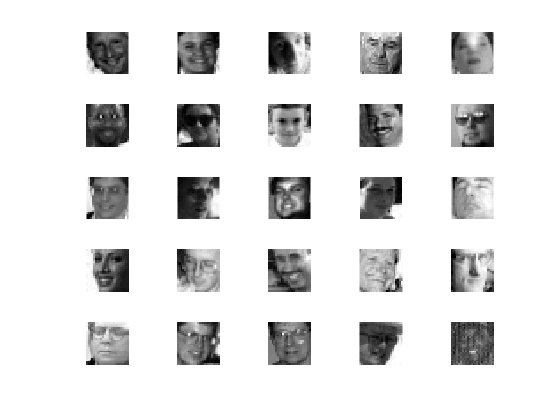
\includegraphics[width=\textwidth]{figures/missclassified_faces.png}
  \end{minipage}
    \begin{minipage}[]{0.8\textwidth}
  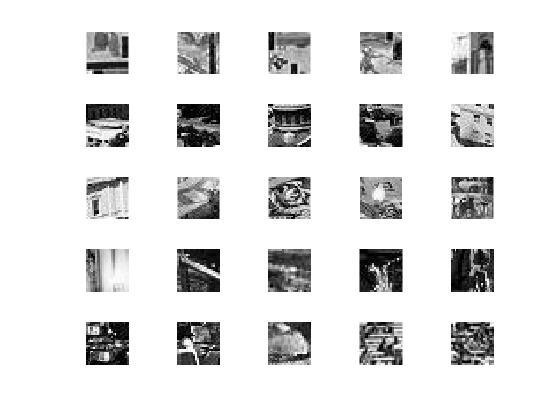
\includegraphics[width=\textwidth]{figures/missclassified_non_faces.png}
  \end{minipage}
\end{figure}

\end{document}
